Space Shuttleの周りの気流の様子を図\ref{fig:result-space}に示す.

\begin{figure}[ht]
    \begin{tabular}{cc}
        \begin{minipage}[b]{0.45\linewidth}
            \centering
            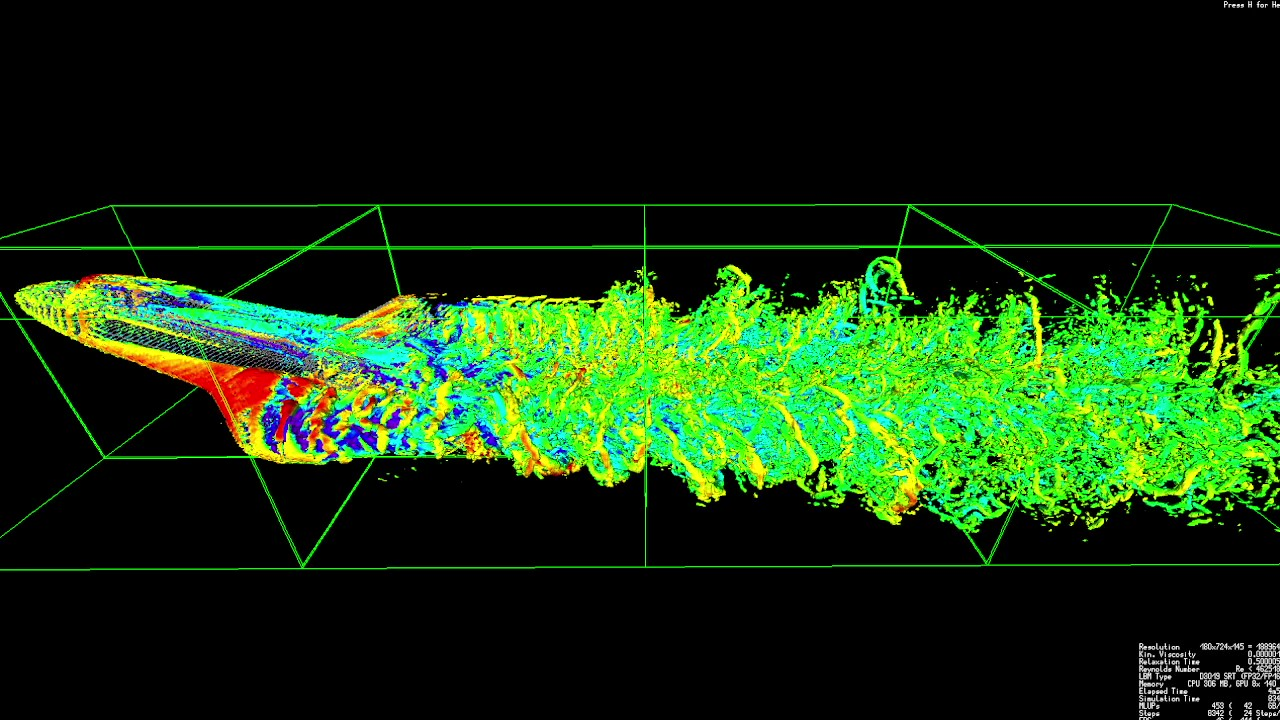
\includegraphics[width=0.9\linewidth]{figures/space/2023-11-05 13-08-17 - frame at 0m0s.jpg}
            \subcaption{\SI{0}{\second}}
        \end{minipage} &
        \begin{minipage}[b]{0.45\linewidth}
            \centering
            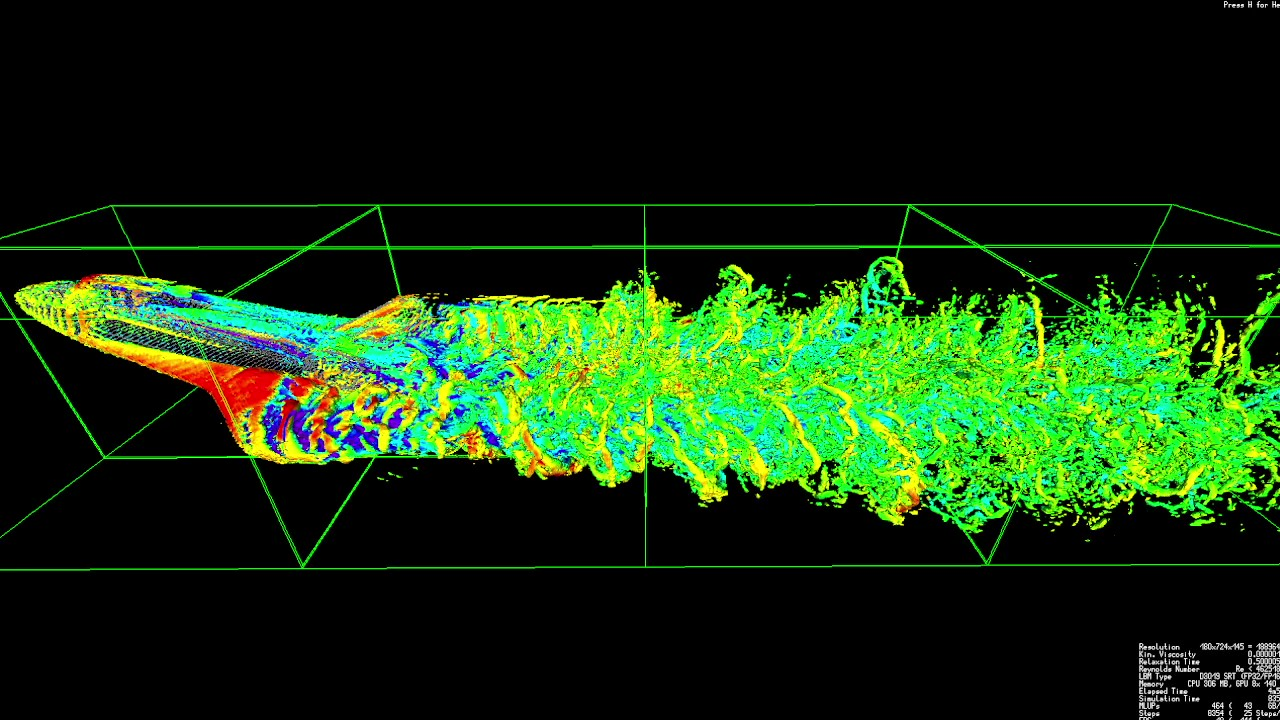
\includegraphics[width=0.9\linewidth]{figures/space/2023-11-05 13-08-17 - frame at 0m1s.jpg}
            \subcaption{\SI{1}{\second}}
        \end{minipage} \\
        \begin{minipage}[b]{0.45\linewidth}
            \centering
            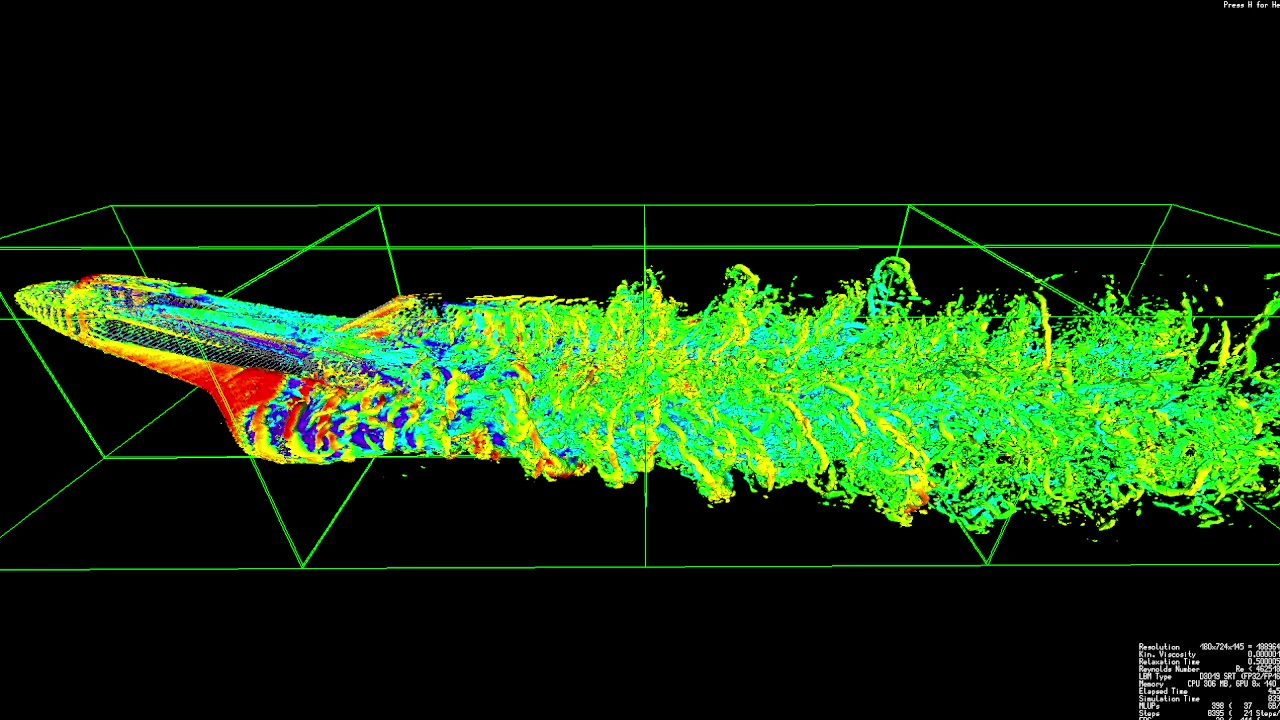
\includegraphics[width=0.9\linewidth]{figures/space/2023-11-05 13-08-17 - frame at 0m2s.jpg}
            \subcaption{\SI{2}{\second}}
        \end{minipage} &
        \begin{minipage}[b]{0.45\linewidth}
            \centering
            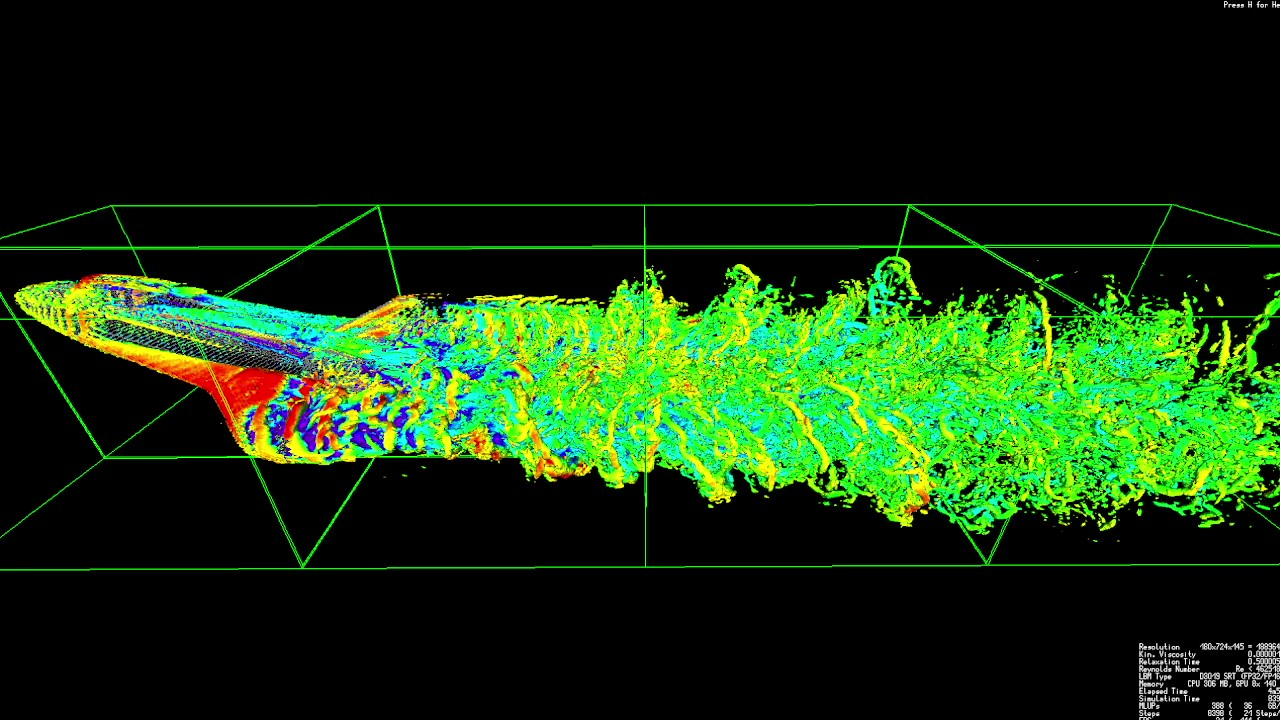
\includegraphics[width=0.9\linewidth]{figures/space/2023-11-05 13-08-17 - frame at 0m3s.jpg}
            \subcaption{\SI{3}{\second}}
        \end{minipage} \\
    \end{tabular}
    \caption{スペースシャトルの周りの気流の様子}
    \label{fig:result-space}
\end{figure}